%%%%% this line is 80 chars wide, please don't make longer lines %%%%%%%%%%%%%%%

\subsection{Rate modulation depth}

\begin{figure*}[ht]
	\centering
  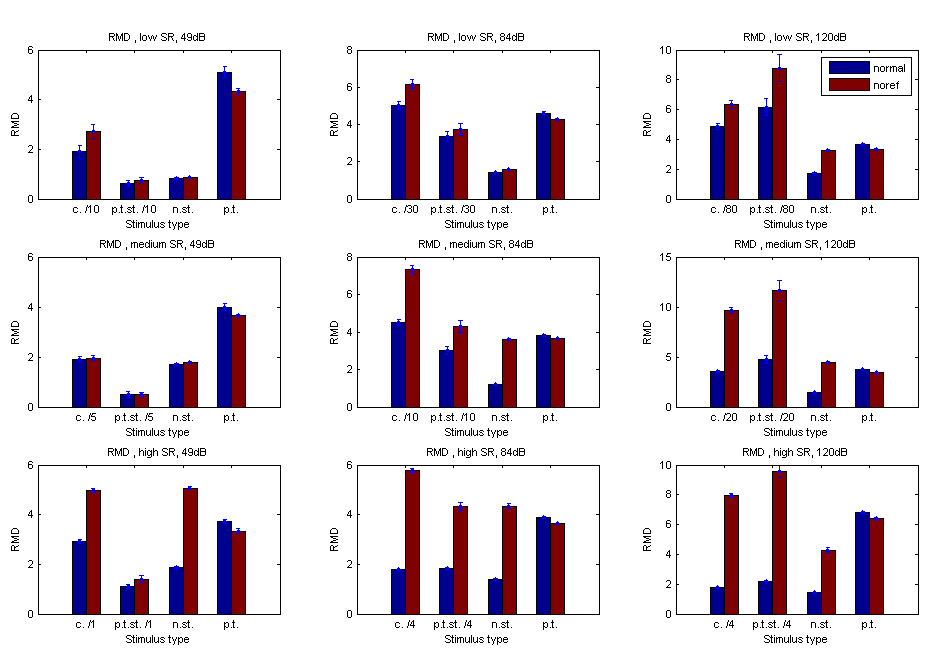
\includegraphics[width=\textwidth]{images/rmds9.png} %or jpg ?; TODO have a better one, and crop it with Paint, see if ok when printed
	\caption{RMD values for different SR fibers and intensities}
	\label{fig:rmds}
\end{figure*}

For the first part of the project, an ad-hoc calculation called rate 
modulation depth (RMD) was used to see difference between encoding 
of acoustic signal with and without absolute refractory period (ARP).

Four kinds of experiments where run and the means of RMD was calculated 
for each of them, 
with each type of nerve fiber, and three different intensities : 
49dB SPL, 84dB SPL and 120dB SPL (49 dB : average home, rainfall, 84 dB : busy road, 120 dB : threshold of discomfort, possible hearing loss) 
% TODO
%http://www.sengpielaudio.com/TableOfSoundPressureLevels.htm; citate ?
%http://noiselimiters.co.uk/buy/noise-levels-what-is-noise.php
to have an overall view of effects.
For every experience, the bin size was 0.01 ms, the characteristic frequency was 1 kHz, 
there was no damage on IHC or OHC, and we told the model to use approximations 
for power-law function calculations. No noise was added to the stimuli.

The four experiments were clicks, pure tones, noise steps and pure tone steps.
The clicks were rarefaction clicks of 0.1 ms and sufficient time was waited between 
two of them to avoid influence from one to the other.
The two steps stimuli had a period of 100 ms and in the first half of the period 
there was noise or pure tone signal, and in the second half there was 0 Pa as pressure.
The noise for the noise step was composed of random normal variables divided 
by the square root of the bin size (gaussian white noise).
The pure tone of the pure tone step was of 10kHz frequency.

We computed then RMD like that : 

$(max - baseline) / baseline$,

where max was 
the maximum of the periodogram of the encoded sounds when converted in 2 ms bins.
The meaning of the baseline depended on the stimulus. 
For the clicks it corresponded to the mean of response to a 0 Pa pressure signal,
 with same number of repetitions than for the click stimulus, to be coherent. 
The noise step has as baseline the value of the periodogram just before the second 
half of the period, so just before the surprise of the sudden change in the stimulus,
 in 10 ms bins. 
The baseline for the pure tone step was the mean of periodogram values
of a response to a pure tone of the frequency used for the stimulus (10 kHz),
after the IHC were saturated, what could be seen in the potential, 
which stays constant because it has not the time 
to be depolarized between two periods of the stimulus. 
The periodogram was computed from the same number of repetitions than for the stimulus, 
like for click baseline, to be coherent with the stimulus.
For the pure tone, the baseline was chosen as the mean of the periodogram.
When baselines for clicks and for pure tone step where computed, 
we took attention to the fact that the number of repetitions of stimulus
for the used periodogram should correspond to the one for the periodogram used for 
calculating the maximum. 
It gives then an equivalent RMD as if we had divided each periodogram by 
their own number of repetitions.

As you can see on \autoref{fig:rmds}, for each type of nerve fiber and 
each decibel value experimented we have similar values in this sense :
for clicks, pure tone steps and noise steps, the RMD without absolute refractory
period is bigger than the normal case, and it is the opposite for pure tones.

%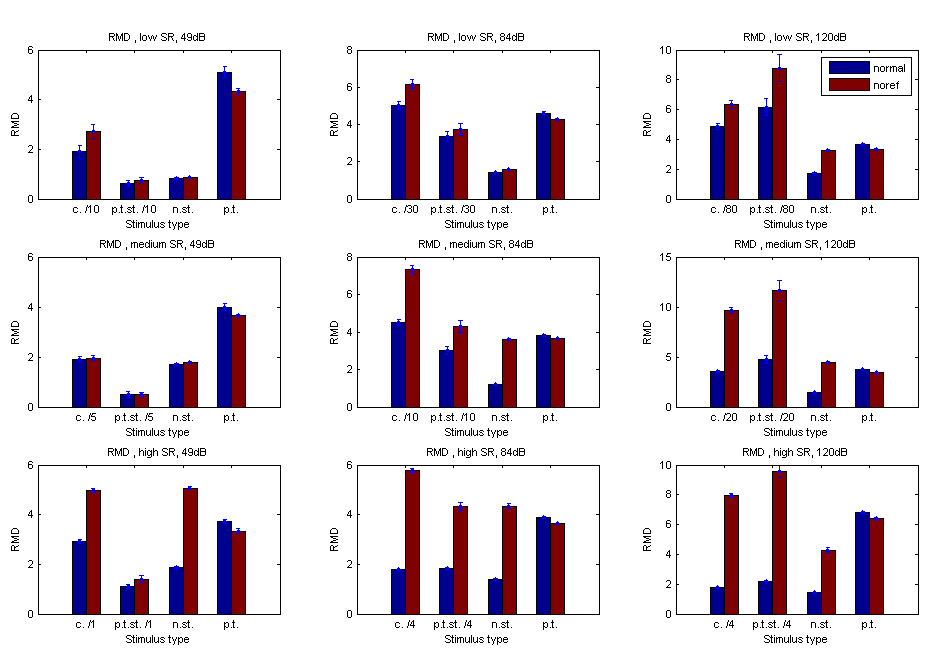
\includegraphics[width=0.45\textwidth]{images/rmds9.jpg}%put higher

We probably can explain the first fact because first, we are in presence of a highly 
non-linear system and, 
secondly, the three stimuli for which the RMD without ARP is bigger than with 
ARP, are stimuli with sudden changes. 
In fact, the click can be seen as an approximation of a delta function, 
which induces a peak in the periodogram just after it, 
and for the steps we have suddenly a signal for some time and suddenly, 
we have no more of it, and that repeatedly, and at each of these changes, 
we have a peak in the periodogram. 
These peaks are then the ones which are used in the RMD computation as the maximum.
In consequence, this RMD result can be interpreted like that : the absolute refractory period 
seems to be able to lower the intensity of the strong response transient induced 
when these kind of sudden changes happens.

%% ! TODO
The second fact, the fact that RMD is lower for pure tones without ARP, 
corresponds to what can be explain by the fact that we have less 
interactions between frequencies in non-linear system,
and with ARP, we have a more non-linear system.

\subsection{Response according to frequencies of modulated pure tones}

In \cite{Deger}, predictions are done for norm and angle of the Fourier coefficients 
(harmonics 0, 1, 2 and 3) of response of stochastic point processes with refractory period,
under modulated pure tone stimuli, with various modulation frequencies.

In fact, the mathematical link between $d$, $d$ being the absolute refractory period,
and the modulation frequency f is of first importance according to the predictions,
 as you can see in \autoref{fig:prednorm} (prediction for the norm of Fourier coefficient) and 
\autoref{fig:predangle} (prediction for its angle). Here d was 80 ms. 
In the graphs, the black ligns are for harmonic 0, dark gray for 1, mid gray for 2, light gray for 3.

%\includegraphics[page=...,viewport=llx lly urx ury,clip]{pdf-file}

\begin{figure}[h]
	\centering
	\includegraphics*[page=4,viewport=308 567 441 617]{images/Deger2010.pdf} %x, y, x, y
	\caption{Predictions for norm (\cite{Deger}  their fig. 3 (c))}
	\label{fig:prednorm}
\end{figure}

\begin{figure}[h]
	\centering
	\includegraphics*[page=4,viewport=433 567 566 617]{images/Deger2010.pdf} %x, y, x, y
	\caption{Predictions for angle (\cite{Deger} their fig. 3 (d))}
	\label{fig:predangle}
\end{figure}
%http://tex.stackexchange.com/questions/40658/extracting-image-from-pdf-to-use-in-latex-document
%pdfimages [options] <PDF-file> <image-root>, on Linux
%http://www.artofproblemsolving.com/Wiki/index.php/LaTeX:Pictures
%http://ctan.org/pkg/graphicx

To see if the predictions are coherent with the model of the peripheral auditory 
system, experiments with modulated pure tone were run. 
The carrier frequency used was 10 kHz, the modulation frequency varied from 50 Hz to 4000 Hz
with steps of 50 Hz. We chose nerve fibers with medium SR, 
and the stimuli were of intensity 84 dB. 
Sadly, not enough data could be yet calculated to see if the results match the prdictions of 
\cite{Deger}.









 